\chapter{Usability Testing}
When we started this project the main reason was to simplify the administration systems to one single interface. So that there is only one code base and only one interface for the user to learn.\\
The first part should be given by default because we use a specialized system to run PHP code on the tablet. The system is called PAW \citep{paw} and is still in its beta phase.\\
The second part is the tricky part. There is only one interface to use, but it must be easy to learn and use so that the system does not have to be reworked.\\
That is why we have performed a usability test.\\
\\

%How did we do the test
	%Who was where
	%The simularity of the questions
\section{Structure of the test}
The test was performed in Cassiopeias usability lab, where we had logged the computer onto our website. The setup of the usability lab is as displayed on figure \ref{fig:usabilitylab}. We did not use the second room.\\
Each test person was lead into the test room, offered a cup of coffee and then we started the prepared briefing, everyone was given the same briefing and we asked them to sign a consent form that they were being tapped for research purposes.\\
After this we asked them to execute a set of assignments within the system, always the same assignments, designed to lead them around the whole active system. \fix{Add a refference to appendix with questions and briefing}\\
We had the same one person sit in the room to assist the user, both to give them their assignment and to tell them when they had completed it. All assignments was kept very short, as to not disturb the user more then needed.\\
When the user had completed all the assignments we had the two men that sat in the control room come and help ask questions to the test person about some of the ways the test person used the system.\\
\\

\begin{figure}[htbp]
	\centering
		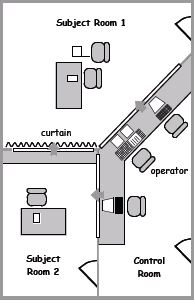
\includegraphics[width=0.40\textwidth]{images/usabilitylab.png}
	\caption{Usability Lab}
	\label{fig:usabilitylab}
\end{figure}

	%Picking the candidates
This test was only performed on 4 persons, this might not sound as many. But being that there is only a few persons in Denmark that will use the administration features that we have designed. We had to make an expert test, and use the gathered data as such. We only had one person available that we thought would use the main system that we have designed, but this person who is responsibly for a kinder garden, is not even high enough up in their system to be using most of the admin features. But this is all we had to go on, as we had no way of contacting the persons who is in a high enough position to be the intended user.\\
So the test was carried out with the one person to be the actual test person, and the 3 others be confirmation test, so that we did not draw conclusions from one test, that could be a result of lacking computer skills or other variables of the same sort.\\
3 out of the 4 test persons is working with kids with autism everyday, and is educated pedagogs, and is therefore very close to the intended user for the administration system, but is in fact the intended user for some of the sub-functionality of the system. The last test person is an educated computer scientist from Aalborg University, whom has a child with autism, this last test persons use of the system was regarded with respect to that of his education and was mainly used for catching really serious bugs and suggestions for new features.\\
\\

	%The old version
Lastly, this test was performed on, at the time, older version of the system. Because of some instabilities in the, at the time, current system. The version that was used for the test can be found on github \citep{testBranch}.\\
\\

\section{Result of the test}
Table \ref{tab:Bugs/Errors} displays the errors or bugs, that we found by the help of the usability test. They are described by first a category, if any, and then by the error itself.\\
They have been sorted by the severity of the error, and we here use 3 categories, critical, serious and cosmetic. Critical depicts an error that either makes a general task impossible or made the user stop all together. Serious depicts an error that made the user stop for some time, or seemed to be unnecessarily distracting. Cosmetic depicts an error of low caliber, that even the users informed us was minor issues that did not affect the flow much more then a few seconds.\\
\\

%Result of the test
	%Bugs/Errors
		%Severity
\begin{table}[htbp]
	\centering
		\begin{tabular}{|l|l|l|}
			\hline
			Description & Severity & Done\\\hline\hline
			It is not possible to create new categories of Pictos & Critical &\\\hline
			Profile - Restrict QR editing to department manager & Critical &  \\\hline 
			DB Problem - Not possible for all pedagogs to fix pictos for all department children & Critical & \\\hline
			Navigation - The site ''Profiles'' should link to each profile & Critical &\\\hline
			Missing - Unable to remove relations & Critical & \\\hline
			Profile Pic - Accept button is hard to find & Serious &\\\hline
			Profile Pic - Word ''change'' is misleading & Serious &\\\hline
			Navigation - ''Add'' and ''Make'' under Pics Manager is confusing & Serious & \\\hline
			Navigation - Language Support on navigation did not change to danish & Serious & Done\\\hline
			Missing - No Danish language support on the site ''Profiles''& Serious &\\\hline
			Profile - Department should be a link, not editable & Serious & (Done)\\\hline
			Profile - Links from Own Profile relations is missing & Serious & \\\hline
			Profile Pic - GIRAF Logo as Placeholder is misleading  & Cosmetic & Done\\\hline
			Profile Pic - Word ''Edit'' is not informative & Cosmetic &\\\hline
			DB Problem - Own Profile takes too long to load & Cosmetic &  \\\hline
			Navigation - ''Add Relation''  is before ''Create Profile'' & Cosmetic & Done \\\hline
			Standardize button names & Cosmetic & \\\hline
			Logout - Can navigate in system without session & Cosmetic & \\\hline
	\end{tabular}
	\caption{Bugs/Errors Found Under Usability Testing}
	\label{tab:Bugs/Errors}
\end{table}

%What have we already fixed
Some of these errors was nearly immediately rectified, or had already been solved in the system that was up to date. These can be seen in table \ref{tab:Bugs/Errors} as ''Done''. If the done, is marked with parentheses, it is because the problem have been partly solved.\\
\\
%What MUST be fixed
As mentioned before there is errors marked critical, as can be seen by the first 5 entries in table \ref{tab:Bugs/Errors}. These are errors that must be fixed for the system to be able to use the implemented features, as listed in chapter \label{chap:systemOverview}.\\
We will here take a moment to explain the critical problems, and in short how they can be rectified.\\
\\
\textbf{It is not possible to create new categories of Pictos}\\
This error arose because we had not thought the creation of categories through. This is one feature that we had overlooked, even after having had a meeting with our contact person, and showing all the features we had intended to create.\\
The way to solve this is to create a minor tool that makes it possible to create and assign categories, that can be created by a simple entry of a text string. For navigation purposes this tool should be put under the Pics Manager category in the navigation menu.\\
\\
\textbf{Profile - Restrict QR editing to department manager}
After having our first test, we was made aware how highly they think of the QR code that they are given for the system. It is supposed to be as important as your house key, and should therefor not be something that can easily be reprinted.\\
Therefor to accommodate this request the QR changer should not be available from the Own Profile site. Instead the procedure will be to contact the admin of the system and have him generate a new key with the QR Manager tool and then send this out.\\
\\
\textbf{DB Problem - Not possible for all pedagogs to fix pictos for all department children}\\
This problem most likely erupted from a misunderstanding between the DB group, WASTELAND, and ourselves. The problem is that in order for a pedagog to edit anything about a child in its department they need to have a relation between them. But this is not how the user intends to use the system. The relation should only be thought of as a responsibility link, and only adds the feature to change this child’s profile data.\\
There is no easy way to rectify this problem from the admin projects side. This has to be fixed inside the database, because of its security mechanisms. For a solution to this we would like the reader to check out the database project, WASTELAND \citep{wasteland}.\\
\\
\textbf{Navigation - The site ''Profiles'' should link to each profile}\\
This is simply a matter of a feature that have not yet been implemented, but it is shown here as an error, because it is necessary for the system to be operated correctly.\\
It can be fixed by adding normal HTML anchor links to each name in the tables.\\
\\
\textbf{Missing - Unable to remove relations}\\
This is again a matter of a feature that have not yet been implemented.\\
We have thought this feature to be usable only for the department manager and the admin of the system. And should be used directly from each users profile. This means that the admin or department manager, navigates to the users profile, and find the person he or she is related to and clicks the button to remove this relation.\\
\\
The rest of the errors is not of a nearly as urgent caliber, and should be easy enough to solve, we will therefore not discuss these further in this report.\\

\section{New Features}
Instead we turn our attention to the possible extra features found during the test, both inspired by the way the users used the system, and their commentary afterward.\\
\\

	%Features
\begin{table}[htbp]
	\centering
		\begin{tabular}{|l|l|}
			\hline
			Description & Done\\\hline\hline
			Make the modal window customizable &\\\hline
			Profile - Press enter to save change &\\\hline
			Pics Manager Make - Add recording feature&\\\hline
			Input forms - Automatic first letter uppercase for name and address&\\\hline  
			Navigation - Add link to ''add relations'' and ''create profile'' in Profiles & \\\hline  
			Pics Manager Make - Directly create picto for child from profile page & \\\hline
			Pics Manager Make - Auto add ''inline-text'' to picto preview & \\\hline
		\end{tabular}
	\caption{Features Found Under Usability Testing}
	\label{tab:NewFeature}
\end{table}	

%What could be added later - Maybe a refference to Future Work instead?
As seen from table \ref{tab:NewFeature} there is a few features that could improve the system. We will here go through some of the features that might be a bit hard to understand without having been on the developing team.\\
\\
\textbf{Make the modal window customizable}\\
We have during this project designed our own modal window, because of some issues with the bootstrap library. It seemed that the user sometimes found it confusing with the many cancel options that is offered for closing the modal window, even though it follows the way bootstrap displays their modal windows.\\
But also in the long run it could be useful to have the ability to customize the modal window with more than a title and a text.\\
\\
\textbf{Input forms - Automatic first letter uppercase for name and address}\\
While watching the users work in the system, we multiple times witnessed them deleting a full text string because they entered the first letter of an address or a name in lowercase. Therefor to save the user time, we thought that making each word in the address and name field automatically convert to uppercase. Since that is the custom with all names and addresses.\\
\\
\textbf{Navigation - Add link to ''add relations'' and ''create profile'' in Profiles}\\
Some of the users in our test meant that the most meaningful way to handle profiles, would be directly from the menu point ''Profiles'', and did not bother to look just below this menu point, where these options lay. This behavior was seen in 3 out of 4 cases, and should therefor be considered.\\
It is a simple addition and does not hinder the system in any way. So if it even only helps a few people in the beginning of the learning of the system, this is feature worth having.
\\
\textbf{Pics Manager Make - Directly create picto for child from profile page}\\
While watching the users work in the system, and also after the, when they were interviewed. We came to understand that some of the pedagogs, in our testcase 2 out of 3. Thought of the child as the central element in the system and therefor wanted to create everything out from the child.\\
This meant that when they had to add parents or pictograms to the child, they went to try and find the child's profile. Therefor in order to accommodate this behavior we should implement a feature that makes it possible to automatically relate a child and a Guardian as well as a child and a pictogram, when the action is started from that child's profile.\\
\\
\textbf{Pics Manager Make - Auto add ''inline-text'' to picto preview}\\
Some of the users did not quite understand what the inline-text field in the Pics Manager Make function meant, before we asked them. Which after they immediately understood what it was for. During the test, we even saw one of our test persons fill the field, and then delete the entry again.\\
If this was a result of the assignment regarding the use of pictograms did not specify that the inline-text field needed to be filled, or something else, we are not certain.\\
But a way to avoid this problem would be to simply add a JavaScript feature that automatically writes on top of the temporary display of the new pictogram.\\
\\
\\
The reader should now be as well informed of the structure and shortcomings of the GIRAF Admin system, as the developer group is. But in case the reader wants more information about the system, the reader should try to contact Ulrik Nyman, Associate Professor at Aalborg University and ask about the GIRAF Admin group of the summer semester, year 2013.\\
In the next chapter we draw conclusions about the system as a whole, and after that we make an evaluation of the process and the multi-project as a whole.


